\subsection{Manifold denoising}

With the assumption of linearity, principal component analysis is a prevailing and efficient method for dimension reduction in high-dimensional space. However, the simple method poses a limitation to respect the nonlinear relationship. 
% Thus, it is essential to develop a powerful and sophisticated approach for nonlinear data analysis. 
Manifold estimation is a technique for modelling the complicated dependence in high-dimensional data, denoising the observations and estimating the low-dimensional latent manifold. Refer to \citet{doi:10.1073/pnas.2311436121} for a detailed review about manifold estimation. 
%Many statistical models have been established to achieve the objective, such as CycleGAN of \citet{doi:10.1073/pnas.2311436121} and principal manifold estimation (PME) of \citet{10.1111/rssb.12416}.

Assume that the observed data $\{x_i\}_{i=1}^m$ is generated from a low-dimensional latent manifold of a high-dimensional ambient space with random noise. That is,
\begin{equation*}
    X=W+\epsilon, \quad X,\epsilon\in \mathbb{R}^D,~W\in \mathbb{M}^d,
\end{equation*}
where $\mathbb{M}^d$ is a $d$-dimensional submanifold of $\mathbb{R}^D$ with $d\leq D$, $W$ is generated from a probability distribution supported in $\mathbb{M}^d$, and $\epsilon$ is $D$-dimensional noise independent of $W$. %The main objective of the manifold estimation is to fit the latent manifold by using $\{x_i\}_{i=1}^m$. According to differentiable geometry, a $d$-dimensional Riemannian manifold with global parametrization is determined by an exponential map $f=(f_1,\ldots,f_D):\mathbb{R}^d\rightarrow \mathbb{M}^d\subset \mathbb{R}^D$, where $\mathbb{R}^d$ is the corresponding tangent space. Therefore, the manifold estimation is also equivalent to finding such a parametrization.
In this article, we propose a two stage manifold estimation (TSME) technique for modelling $\mathbb{M}^d$. The primary challenge of parametrization is attributed to the lack of the required pairs of training data, \emph{i.e.}, (predictor, response). %Thus, it is an unsupervised learning problem. 
We resolve the issue simply by combining the manifold embedding and reconstruction. The manifold embedding is a nonlinear dimensional reduction method. Many impressive algorithms have been proposed in the literature, such as ISOMAP \citep{balasubramanian2002isomap}, Laplacian eigenmaps \citep{belkin2003laplacian} and UMAP \citep{mcinnes2018umap}. 

At the first stage, we apply the manifold embedding technique in $\{x_i\}_{i=1}^m$ given the intrinsic dimension $d$, yielding a projection map $\hat{g}:\mathbb{R}^D\rightarrow \mathbb{R}^d$. Let $u_i=\hat{g}(x_i)$ for $i=1,\ldots,m$. Then $\{(u_i,x_i)\}_{i=1}^m$ are the training samples for the manifold reconstruction. At the second stage, we execute the regression in $\{(u_i,x_i)\}_{i=1}^m$ to reconstruct the manifold. For example, we can use the proposed EBARS method to estimate the reconstruction map $\hat{f}$. Due to the automatic knot selection, EBARS is eligible to model the complex relationships between $u$ and $x$. Consequently, the manifold estimation is completed by the composition of the embedding $\hat{g}$ and the reconstruction $\hat{f}$. Especially, $\{\hat{f}\circ \hat{g}(x_i)\}_{i=1}^m$ can serve as the denoised representation of $\{x_i\}_{i=1}^m$. %Furthermore, the composition $\hat{f}\circ\hat{g}$ can be considered as a solution to the minimum problem of the loss function $\mathbb{E}\left|\left| X-f\circ g(X) \right|\right|^2$.

We conduct the TSME method in manifold denoising and compare its performance with MFUN, PMF, PME and PC. Notably, PME and PC adopt a similar framework with our TSME except that they utilize smoothing splines for reconstruction. The data is generated from two disconnected arcs in $\mathbb{R}^2$, a spiral curve in $\mathbb{R}^2$ and a Swiss roll in $\mathbb{R}^3$, as shown in Figures \ref{fig:d1} and \ref{fig:d2}.%corresponding to $(d=1,D=2)$ and $(d=2,D=3)$. 
ISOMAP is used as the embedding map of TSME and the initial projection of PME in the spiral and  Swiss roll. For the arc case, we substitute UMAP for ISOMAP due to the disconnectivity. Besides, for the Swiss roll, we only compare TSME, MFUN and PMF, as PC is limited to the curve case and PME is very slow with disastrous performance. The random noise is Gaussian with standard deviation $0.2,0.2,1.5$.

Simulation results including the training samples and the denoised data are visualized in Figures \ref{fig:d1} and \ref{fig:d2}. The sample sizes are $m=1000,1500,3000$. Compared with TSME, the PME and PC methods collapse dramatically in curve cases. In arcs, the disconnectivity of $\mathbb{M}^d$ causes the jumping discontinuity of the reconstruction map. %As mentioned above, EBARS is superior to the smoothing splines in describing sharp changes. 
In spiral, the dependency is complex due to the intricate manifold, posing a critical challenge in selecting the optimal penalty weight of smoothing splines. %And the smoothness in EBARS is controlled based on the number of knots without the penalty term. 
For MFUN and PMF, the denoised representations remain corrupted in the spiral and Swiss roll cases. They don't mitigate the random noise successfully and fail to estimate the latent manifolds accurately.

\begin{figure}
    \centering
    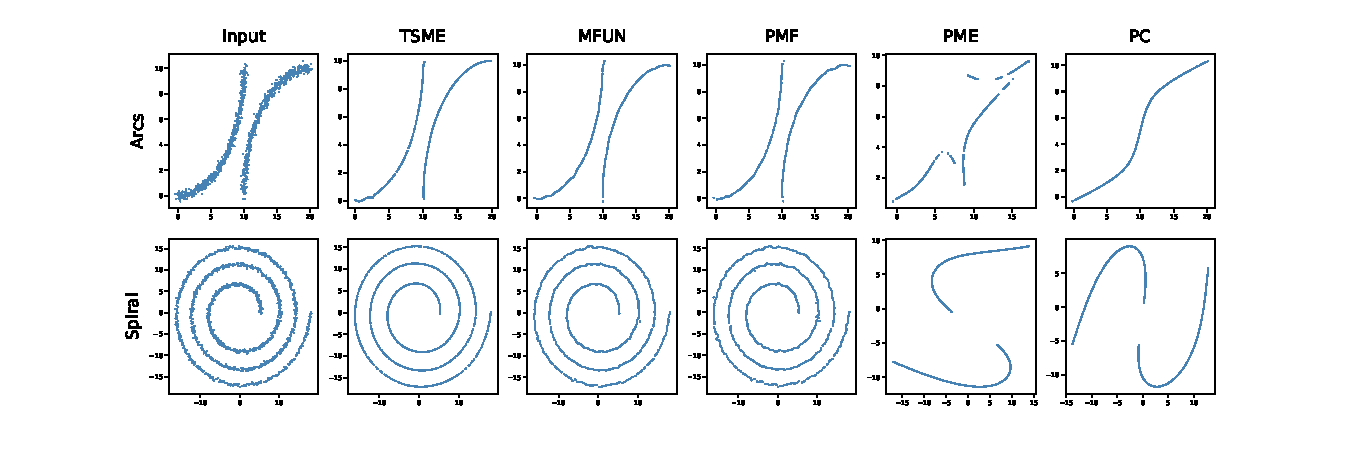
\includegraphics[width=0.9\textwidth]{Experiments/plots/crop_dim1.pdf}
    \caption{Manifold denoise results for two curve scenarios. Each plot indicates the training samples or the denoised representation obtained by our TSME, MFUN, PMF, PME and PC.}
    \label{fig:d1}
\end{figure}

\begin{figure}
    \centering
    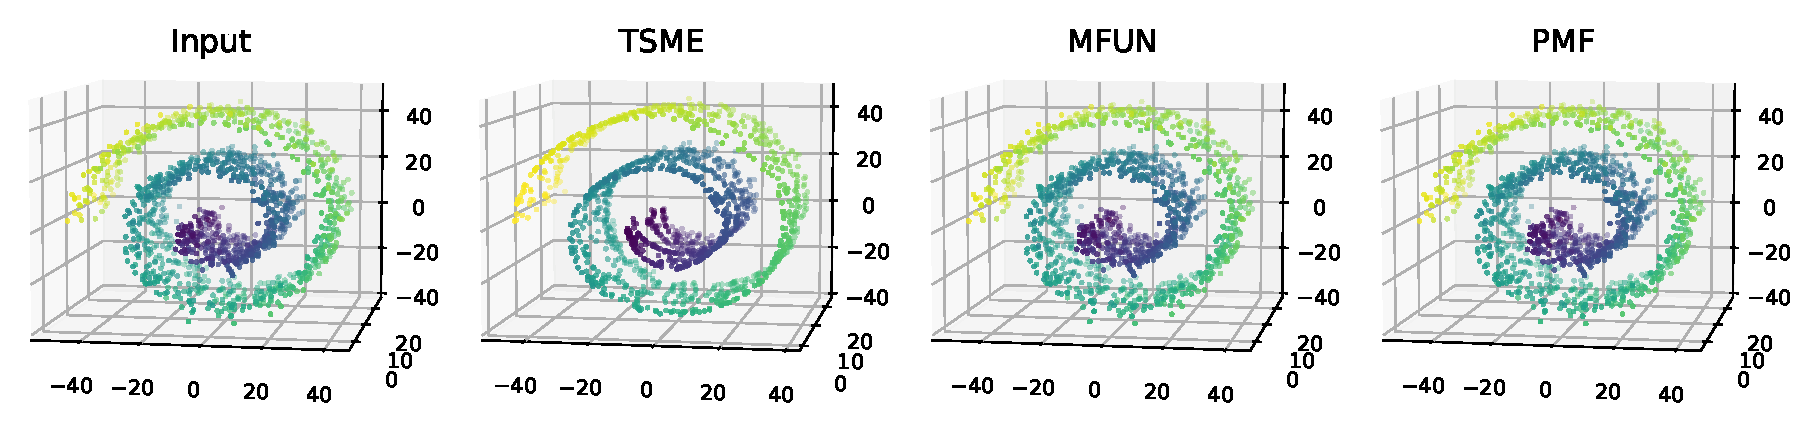
\includegraphics[width=0.95\textwidth]{Experiments/plots/dim2.pdf}
    \caption{Manifold denoise results for the Swiss roll. Each plot indicates the training samples or the denoised representation obtained by our TSME, MFUN and PMF.}
    \label{fig:d2}
\end{figure}

To evaluate the performance quantitatively, we define the geometric mean squared distance as
\begin{equation*}
    \text{GMSD}=\frac{1}{m}\sum_{i=1}^m \text{dist}(\hat{f}\circ\hat{g}(x_i),\mathbb{M}^d)^2,
\end{equation*}
where $\text{dist}(x,\mathbb{M}^d)=\inf_{x'\in\mathbb{M}^d}||x-x'||$. The GMSD measures the corrupted extent of the data away from the manifold. Table \ref{tab:gmsd} illustrates the mean and standard deviation of GMSD in three manifolds of $20$ duplicates. TSME obtains significantly smaller GMSD than the training samples in all scenarios and achieves the smallest GMSD in most cases, demonstrating that our method contributes to excellent manifold denoising. For MFUN and PMF, the performance in the $d=1$ cases is satisfactory but the noise is not reduced in the Swiss roll. PME and PC are completely incapable of estimating the latent manifolds. %This indicates again the great advantage of EBARS over the smoothing spline with equally-spaced fixed knots.

\begin{table}
    \centering
    \caption{Summary of GMSD with respect to five methods in three manifolds}
    \label{tab:gmsd}
    \begin{tabular}{@{}cccc@{}}
    \toprule
          & Arcs                    & Spiral                  & Swiss roll              \\ \midrule
    $m$ & 500 & 1000 & 1500 \\
    Input & 0.0404(0.0020)          & 0.0397(0.0021)          & 2.6033(0.0729)          \\
    TSME  & 0.0036(0.0021)          & 0.0019(0.0003) & 0.5299(0.0653) \\
    MFUN  & 0.0039(0.0011) & 0.0112(0.0011)          & 2.5549(0.0735)          \\
    PMF   & 0.0051(0.0011)          & 0.0165(0.0017)          & 2.5994(0.0733)          \\
    PME   & 0.4790(0.2585)          & 2618.6(9887.4)          &            $\times$             \\
    PC    & 0.7661(0.0077)          & 2.9539(0.0633)          &            $\times$             \\ \midrule
        $m$ & 1000 & 1500 & 3000 \\
    Input & 0.0399(0.0013)          & 0.0401(0.0013)          & 2.6423(0.0621)          \\
    TSME  & 0.0044(0.0033)          & 0.0015(0.0002) & 0.5004(0.0605) \\
    MFUN  & 0.0018(0.0004) & 0.0078(0.0005)          & 2.5377(0.0629)          \\
    PMF   & 0.0023(0.0007)          & 0.0113(0.0008)          & 2.6241(0.0625)          \\
    PME   & 0.3135(0.1353)          & 151.87(449.52)          &            $\times$             \\
    PC    & 0.7589(0.0072)          & 2.9601(0.0699)          &            $\times$             \\ 
    \bottomrule
\end{tabular}
\end{table}


\iffalse
The so-called principal manifold is the minimizer of the following objective function in a well-defined functional space,
\begin{equation}
\label{eq:pme}
    \mathbb{E}\left|\left| X-f(\pi_f(X)) \right|\right|^2 + \lambda \sum_{l=1}^D \int_{\mathbb{R}^d} \sum_{i,j=1}^d \left|\frac{\partial^2 f_l}{\partial t_i \partial t_j}(t)\right|^2 dt,
\end{equation}
where $\lambda$ is the penalty weight, $f:\mathbb{R}^d\rightarrow \mathbb{M}^d \subset \mathbb{R}^D$ is equivalent to the exponential map and $\pi_f:\mathbb{R}^D\rightarrow \mathbb{R}^d$ is the corresponding projection. The PME algorithm solves \eqref{eq:pme} in an iterative fashion. That is, given an initial estimation, $f_{n+1}=\arg \min  \mathbb{E}\left|\left| X-f(\pi_{f_n}(X)) \right|\right|^2 + \text{penalty}$. \citet{10.1111/rssb.12416} utilizes thin plate splines to compute $f_{n}$ with $\pi_{f_0}$ given by ISOMAP \citep{balasubramanian2002isomap}. In this example, we substitute EBARS for thin plate splines to estimate manifolds and compare their performance. In addition, the practice suggests that more iteration steps have little effect on the improvement. Thereby we just update one step. Consequently, the overall manifold fitting algorithm is to solve the least-square problem $\frac{1}{m}\sum_{i=1}^m ||x_i-f(\pi_{f_0}(x_i))||^2$, where $\{x_i\}_{i=1}^m\subset \mathbb{R}^D$ are data samples and $f$ is estimated by EBARS.

The data involved is illustrated in Column 1 of Figure \ref{fig:manifold_fitting}. It consists of the spiral curve in $\mathbb{R}^2$, the space spiral in $\mathbb{R}^3$ and the Swiss roll in $\mathbb{R}^3$, corresponding to $(d=1,D=2)$, $(d=1,D=3)$ and $(d=2,D=3)$ respectively. The noise is Gaussian with standard deviation $0.35,0.4,0.5$. The sample sizes for the three cases are $1000,1000,2000$. The estimated manifolds are visualized in Columns 2 and 3 of Figure \ref{fig:manifold_fitting}. The PME method collapses dramatically due to the complex intrinsic structures, leading to meaningless manifolds as shown in Column 3. On the contrary, it is surprising to find that the EBARS method fits excellent latent manifolds in three cases as shown in Column 2. The primary reason is that the optimal choice of $\lambda$ in \eqref{eq:pme} causes a challenge for the PME algorithm, whereas it doesn't involves any penalty in EBARS. The impressive results again indicate great advantages of EBARS over equally-spaced knot splines.


\begin{figure}[ht]
    \centering
    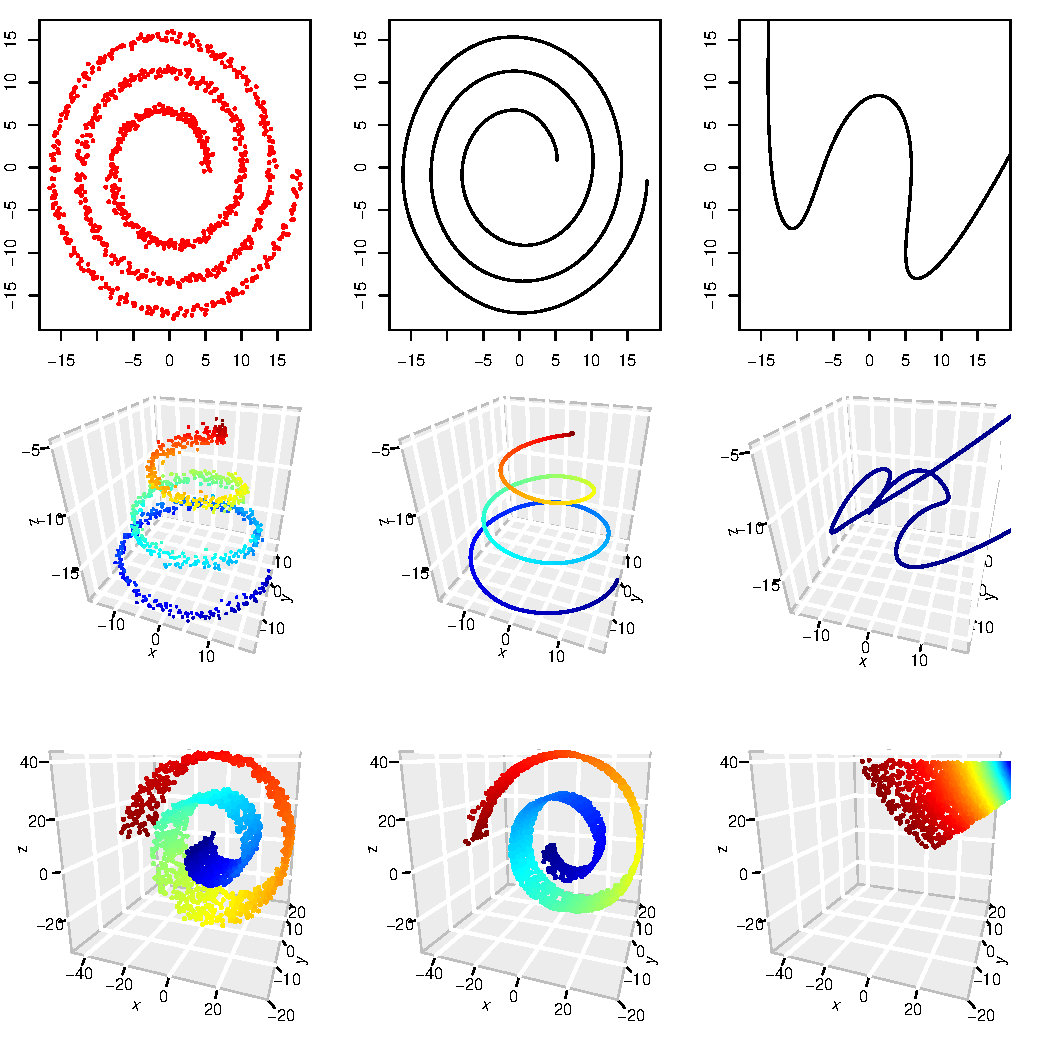
\includegraphics[width=1\textwidth]{Experiments/plots/manifold_fitting.pdf}
    \caption{Manifold fitting for spiral curves in $\mathbb{R}^2$ and $\mathbb{R}^3$ and Swiss roll in $\mathbb{R}^3$. Column 1: the ground truth. Column 2: fitting by EBARS. Column 3: fitting by PME.}
    \label{fig:manifold_fitting}
\end{figure}
\fi